\documentclass[12pt]{article}

\usepackage[utf8]{inputenc}
\usepackage[greek,english]{babel}
\usepackage[unicode]{hyperref}
\usepackage{alphabeta}
\usepackage{amsmath}
\usepackage{mathtools}
\newcommand{\Lagr}{\mathcal{L}}
\usepackage{graphicx}
\usepackage{bookmark}
\usepackage{amsfonts}
\setlength{\arrayrulewidth}{1mm}
\setlength{\tabcolsep}{18pt}
\renewcommand{\arraystretch}{1.5}
 
\begin{document}

\author{Κωνσταντίνος Λέτρος 8851}

 \begin{titlepage} % Suppresses displaying the page number on the title page and the subsequent page counts as page 1
	\newcommand{\HRule}{\rule{\linewidth}{0.5mm}} % Defines a new command for horizontal lines, change thickness here
	
	\center % Centre everything on the page
	
	%------------------------------------------------
	%	Headings
	%------------------------------------------------
	
	\textsc{\LARGE ΠΟΛΥΤΕΧΝΙΚΗ ΣΧΟΛΗ ΑΠΘ}\\[1.5cm] % Main heading such as the name of your university/college
	
	\textsc{\Large ΤΜΗΜΑ ΗΛΕΚΤΡΟΛΟΓΩΝ ΜΗΧΑΝΙΚΩΝ ΚΑΙ ΜΗΧΑΝΙΚΩΝ ΥΠΟΛΟΓΙΣΤΩΝ}\\[0.5cm] % Major heading such as course name
	
	 
	
	%------------------------------------------------
	%	Title
	%------------------------------------------------
	
	\HRule\\[0.4cm]
	
	{\huge\bfseriesΠροσομοίωση και Μοντελοποίηση Συστημάτων}\\[0.4cm] % Title of your document
	
	\HRule\\[1.5cm]
	
	%------------------------------------------------
	%	Author(s)
	%------------------------------------------------
	{\huge\bfseries Κωνσταντίνος Λέτρος \newline 8851}\\[0.4cm]	
	\vfill	
	{\huge\bfseries Project}\\[0.4cm]  % Title of your document
	% If you don't want a supervisor, uncomment the two lines below and comment the code above
	%{\large\textit{Author}}\\
	%John \textsc{Smith} % Your name
	
	%------------------------------------------------
	%	Date
	%------------------------------------------------
	
	\vfill\vfill\vfill % Position the date 3/4 down the remaining page
	
	{\large\today} % Date, change the \today to a set date if you want to be precise
	
	%------------------------------------------------
	%	Logo
	%------------------------------------------------
	
	%\vfill\vfill
	%\includegraphics[width=0.2\textwidth]{placeholder.jpg}\\[1cm] % Include a department/university logo - this will require the graphicx package
	 
	%----------------------------------------------------------------------------------------
	
	\vfill % Push the date up 1/4 of the remaining page
	
\end{titlepage}





\newpage
\part*{Αναγνώριση Αγνώστου Γραμμικού Συστήματος}
\section{Εισαγωγή}
Δίνεται άγνωστο σύστημα ΜΕΜΕ (Μίας Εισόδου - Μίας Εξόδου) με μοναδικά μετρήσιμα σήματα την είσοδο και έξοδό του. Στόχος μας είναι η μοντελοποίηση του συστήματος κατά μαύρο κουτί.
\\ \\
Αρχικά θα επιβεβαιώσουμε ότι το άγνωστο σύστημα ΜΕΜΕ, του οποίου τις παραμέτρους θέλουμε να βρούμε, είναι ΓΧΑ (Γραμμικό και Χρονικά Αμετάβλητο). Οι έλεγχοι που παρουσιάζονται υλοποιήθηκαν στο αρχείο LTICheck.m .
\subsection{Έλεγχος Γραμμικότητας}
Για να είναι το σύστημα γραμμικό θα πρέπει να ισχύει η αρχή της υπέρθεσης, δηλαδή για οποιεσδήποτε εισόδους $u_1,u_2$ και σταθερές $c_1 ,c_2 $ να ισχύει
\[y \left(t;0,c_1 u_1+ c_2 u_2, \right)=c_1 y(t;0,u_1) + c_2 y(t;0,u_2 ) \]
Έτσι επιλέγουμε τυχαία δύο εισόδους για το σύστημα
\[ u_1(t)=sin(t)+2cos(3t)+5cos(7t)+9sin(10.5t) \] και 
\[ u_2(t)=12cos(3.5t)+15sin(2.5t) + cos(2t) \]
που έχουν αποκρίσεις $y_1(t)$ και $y_2(t)$ αντίστοιχα και $c_1 ,c_2 $ τυχαία επιλεγμένες σταθερές.
Θέτουμε 
\[ y_{12}(t)=c_1y_1(t)+c_2y_2(t)\]
Στη συνέχεια επιλέγουμε ως είσοδο $u_3(t)$ το άθροισμα
\[ u_3(t)=c_1u_1(t)+c_2u_2(t) \]
οπότε το σύστημα έχει απόκριση $y_3(t)$. Τέλος, υπολογίζουμε το σφάλμα
\[e_{1}(t)=y_3(t)-y_{12}(t)\]
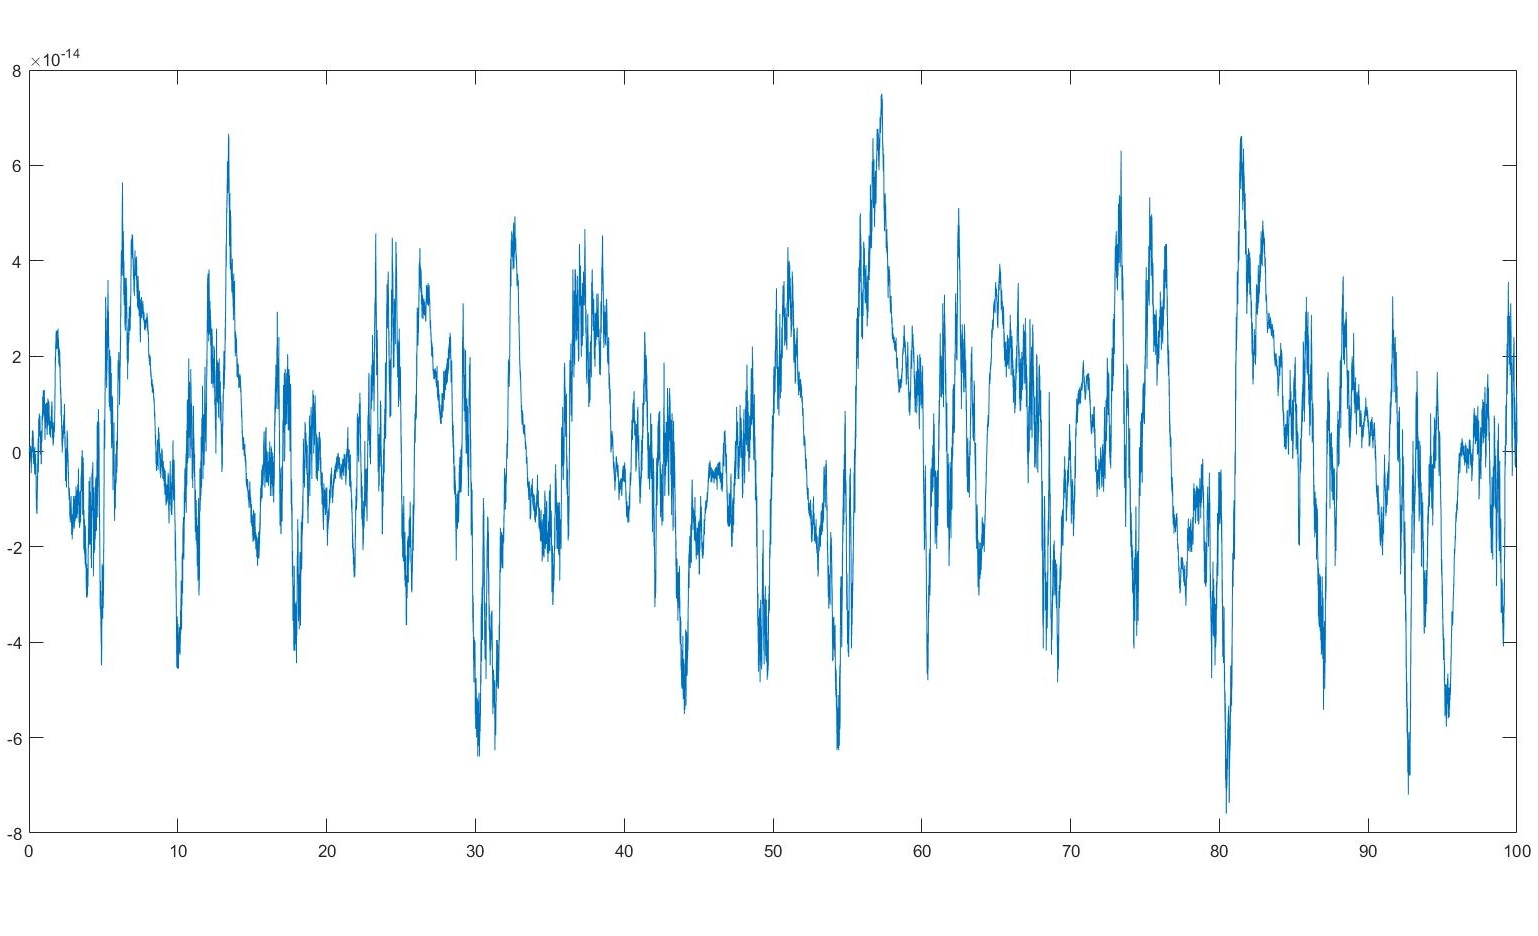
\includegraphics[width=\linewidth]{linear.jpg}
\centerline{Σχήμα 1.1:  Έλεγχος Γραμμικότητας}
\centerline{του Άγνωστου Συστήματος}
\\ \\ \\
το οποίο είναι της τάξης του $10^{-14}$ δηλαδή πρακτικά μηδενικό. 
\subsection{Έλεγχος Χρονικής Αμεταβλητότητας}
Για να έιναι ένα σύστημα χρονικά αμετάβλητο θα πρέπει για οποιαδήποτε είσοδο $u$ και σταθερά $t_0$ να ισχύει
\[u(t) \rightarrow y(t) \Rightarrow u(t-t_0) \rightarrow y(t-t_0)\]
Επομένως για να κάνουμε αυτό τον έλεγχο, επιλέγουμε τυχαία μια είσοδο $u_1$
\[ u_1(t)=cos(t)+3sin(5t)+8cos(8t)+3sin(15t)\]
και υπολογίζουμε την έξοδο $y_1$. Στη συνέχεια επιλέγουμε την είσοδο
\[ u_2(t)=u_1(t-t_0)=cos(t)+3sin[5(t-t_0)]+8cos[8(t-t_0)]+3sin[15(t-t_0)] \]
και υπολογίζουμε την έξοδο $y_2$, όπου το $t_0$ επιλέγεται τυχαία σε κάθε εκτέλεση του αλγορίθμου. Τέλος υπολογίζουμε το σφάλμα
\[e_{2}(t)=y_1(t-t_0)-y_2(t) \]
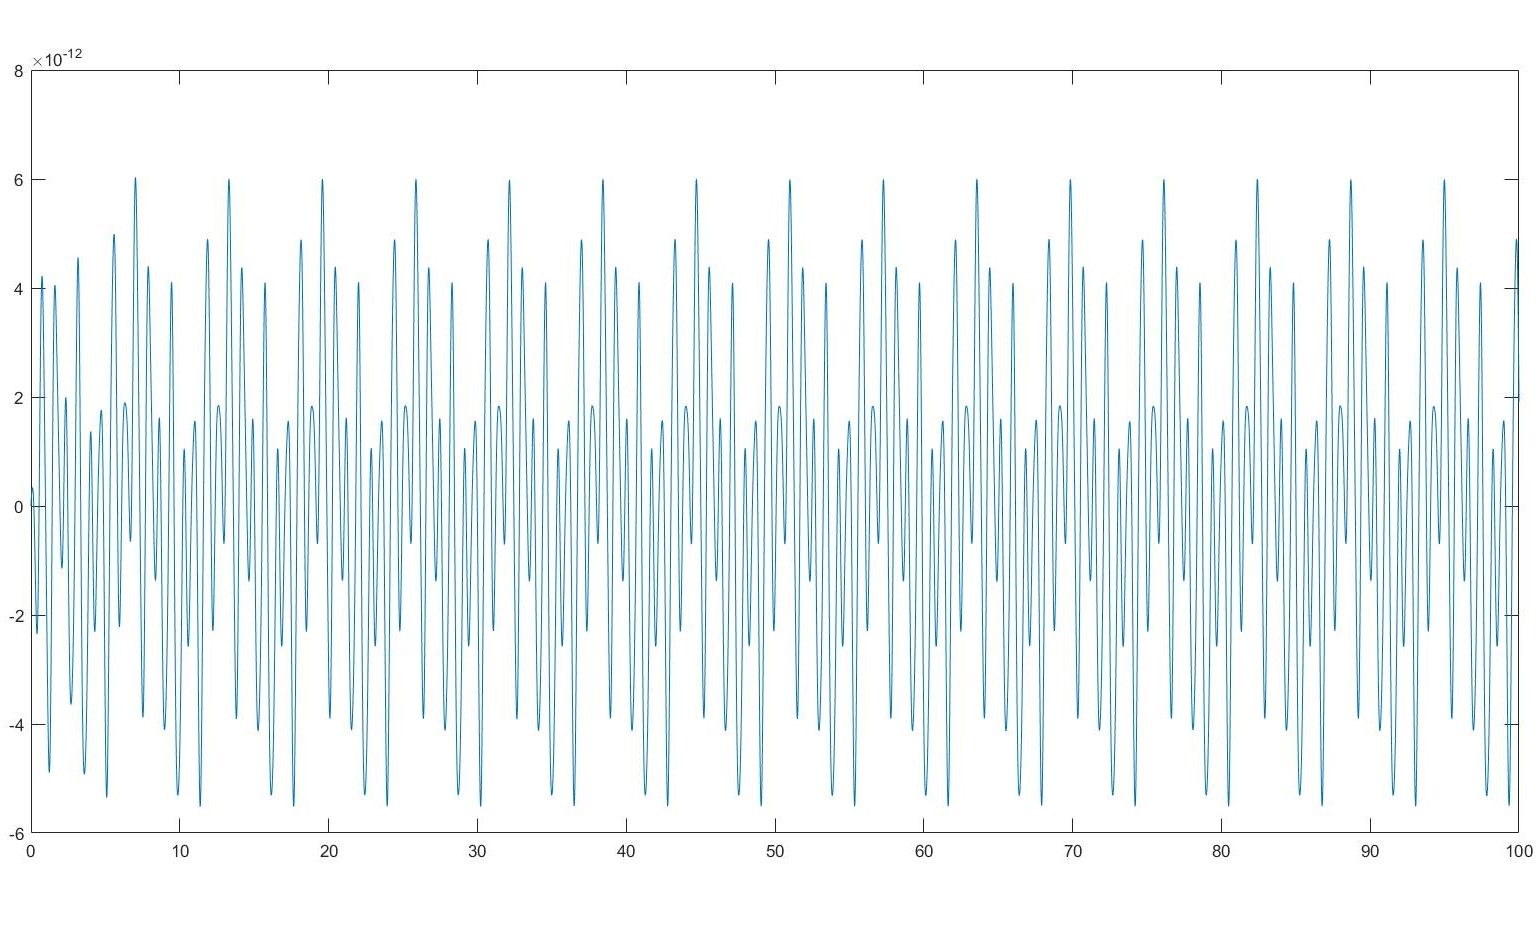
\includegraphics[width=\linewidth]{time_inv.jpg}
\centerline{Σχήμα 1.2: Έλεγχος Χρονικής Αμεταβλητότητας}
\centerline{του Άγνωστου Συστήματος}
\\ \\ \\
το οποίο είναι της τάξης του $10^{-12}$ δηλαδή κι αυτό πρακτικά μηδενικό. 
\\ \\
Οι παραπάνω έλεγχοι έγιναν για πολλές και διαφορετικές εισόδους με περισσότερους όρους, καθώς επίσης και για πολύ μεγαλύτερα χρονικά διαστήματα (κάποιων ωρών) και τα αποτελέσματα ήταν παρόμοια.
\section{Επιλογή Μεθόδου Εκτίμησης}
Αφού το σύστημα είναι Γραμμικό και Χρονικά Αμετάβλητο,  περιγράφεται από τη γραμμική διαφορική εξίσωση, της μορφής
\\
\[ y^{(n)}+a_1y^{(n-1)}+...+a_{n-1}\dot{y}+a_{n}y=b_0 u^{(m)}+b_1u^{(m-1)}+...+b_{m-1}\dot{u}+b_{m}u \Leftrightarrow\]
\[ y^{(n)}=-a_1y^{(n-1)}-...-a_{n-1}\dot{y}-a_{n}y+b_0 u^{(m)}+b_1u^{(m-1)}+...+b_{m-1}\dot{u}+b_{m}u \quad (1)\]
\\
όπου όπως βλέπουμε από την απόκριση για μηδενική εισόδο, έχει μηδενικές αρχικές συνθήκες και για το οποίο θέλουμε να εκτιμήσουμε τις παραμέτρους $a_i$ και $b_j$ με $i=1,2,...,n$ και $j=0,1,...,m$.
\\ \\
Για το σκοπό αυτό επιλέχθηκαν διάφορα μοντέλα, δηλαδή διαφορετικές τιμές των $n,m$ και χρηισμοποιηθήκαν οι offline και online μέθοδοι ελαχίστων τετραγώνων.
\\ \\
Για τη λειτουργία του αλγορίθμου εκτελούμε το αρχείο main.m όπου επιλέγονται οι τιμές των $n$ και $m$ και στη συνέχεια οι (θετικοί) συντελεστές του ευσταθούς φίλτρου $\Lambda(s)$ που εμφανίζεται στη μέθοδο, όπως παρουσιάζεται στη συνέχεια (μέχρι n=5, ωστόσο μπορούν να προστεθούν κι άλλα φίλτρα χωρίς να επηρρεαστεί η καλή λειτουργία του αλγορίθμου).
\subsection{Offline Μέθοδος Ελαχίστων Τετραγώνων}
\subsubsection{Θεωρητική Ανάλυση}
Μπορούμε να γράψουμε τη διαφορική εξίσωση $\left(1\right)$  με τη μορφή \quad $\dot{y}=\theta^{*T}\Delta$ \quad όπου
\[\theta_{1}^{*}=
\begin{bmatrix}
		a_1 & a_2 & ... & a_n
\end{bmatrix}^{T}
\qquad
\theta_{2}^{*}=
\begin{bmatrix}
		b_0 & b_1 & ... & b_m
\end{bmatrix}^{T}
\qquad
\theta^{*}=
\begin{bmatrix}
		\theta_{1}^{*T} & \theta_{2}^{*T}
\end{bmatrix}^{T}
\]
και 
\[ \Delta=
\begin{bmatrix}
	-y^{(n-1)} & ...  & -\dot{y} & -y & u^{(m)} & ...  & \dot{u} & u
\end{bmatrix}^{T} \]
ή στο πεδίο Laplace
 \[ \Delta(s)=
\begin{bmatrix}
		 -s^{n-1}Υ(s) & ... & -sΥ(s) & -Υ(s) & s^{m}U(s) & ... & sU(s) & U(s)
\end{bmatrix}^{T} =\]
\[ \begin{bmatrix}
		-\Delta_{n-1}^{T}(s)Υ(s) & \Delta_{m}^{T}(s)U(s)
\end{bmatrix}^{T}\]

Ωστόσο, δεν γνωρίζουμε-μετράμε τις τιμές των παραγώγων του $y(t)$. Οπότε, για να μπορέσουμε να προχωρήσουμε, θεωρούμε ευσταθές πολυώνυμο $\Lambda(s)$  (όλες του οι ρίζες ανήκουν στο αριστερό μιγαδικό ημιεπίπεδο) στο πεδίο $Laplace$ n-στου βαθμού, \quad $\Lambda(s)=s^{n}+s^{n-1}\lambda_1+...+s\lambda_{n-1}+\lambda_n$ \quad (με θετικούς συντελεστές) ώστε με τη χρήση του φίλτρου $1/\Lambda(s)$ να φιλτράρουμε την έξοδο. Γι'αυτό ορίζουμε τον πίνακα $\lambda$.
\[ \lambda= \begin{bmatrix}
\lambda_1 & ... & \lambda_{n-1} & \lambda_n
\end{bmatrix}^{T} \]
Έτσι, το σύστημα μπορεί να παραμετροποιηθεί γραμμικά και να γραφτεί στη μορφή γραμμικής οπισθοδρόμησης \quad  $y=\theta^{T}_{\lambda}\zeta$ \quad  στο πεδίο του χρόνου ή στο πεδίο $Laplace$ ως \quad $Y(s)=\theta^{T}_{\lambda}\zeta(s)$ \quad όπου $\zeta$ το διάνυσμα οπισθοδρόμησης.
\[\theta_{\lambda}=\begin{bmatrix}
		\theta_{1}^{*T}-\lambda^{Τ} \quad& \theta_{2}^{*T}
\end{bmatrix}^{T}\]
και
\[
\zeta(s)=\begin{bmatrix}
		-\frac{\Delta^{T}(s)Υ(s)}{\Lambda(s)} & \frac{\Delta^{T}(s)U(s)}{\Lambda(s)}
\end{bmatrix}^{T} \]
Επομένως \quad 
\[Υ(s)=
\begin{bmatrix}
		\theta_{1}^{*T}-\lambda^{Τ} \quad& \theta_{2}^{*T}
\end{bmatrix}
\begin{bmatrix}
		-\frac{\Delta^{T}(s)Υ(s)}{\Lambda(s)} & \frac{\Delta^{T}(s)U(s)}{\Lambda(s)}
\end{bmatrix}^{T} \]
και επιστρέφοντας στο πεδίο του χρόνου\quad $y(t)=\Lagr^{-1}(Y(s))$ 
\\ \\
Στη συνέχεια θα χρησιμοποιήσουμε τη μέθοδο ελαχίστων τετραγώνων με στόχο να ελαχιστοποιήσουμε το σφάλμα εκτίμησης και τελικά να εκτιμήσουμε με σχετική ακρίβεια τις επιθυμητές παραμέτρους. Για το σκοπό αυτό θεωρούμε τη συνάρτηση σφάλματος $e$.
\\
\[e=y-\hat{y}=y-\hat{\theta}^{T}_{\lambda}\phi\]
\\
 όπου με $\hat{\theta}$ και $\hat{y}$ συμβολίζονται οι εκτιμήσεις των $\theta$ και $y$ αντίστοιχα και $\phi$ ο πίνακας που περιέχει τις αριθμητικές τιμές του διανύσματος οπισθοδρόμησης $\zeta$.
\\ \\
Έπειτα επιδιώκουμε να ελαχιστοποιήσουμε την $K(\hat{\theta})=\frac{1}{2}e^2$ , η οποία είναι κυρτή συνάρτηση (κάθε τοπικό ελάχιστο είναι και ολικό ελάχιστο) ως προς $\hat{\theta}$.
Για να έχουμε την ελάχιστη τιμή \quad $min_{\hat{\theta}} K(\hat{\theta})$ λύνουμε την εξίσωση
\\ 
\[  \nabla_{\hat{\theta}} K(\hat{\theta}) \Bigr|_{\substack{\hat{\theta} =\theta_{0}}}=0 \]
 \\
 από όπου προκύπτει 
 \[
 \phi\phi^{T}\theta_{0}=\phi y
\] 
 \\ 
και τέλος λύνουμε το παραπάνω σύστημα για να βρούμε το $\theta_{0}$. Όταν ελαχιστοποιείται το σφάλμα, έχουμε
 \\
\[ e \approx 0 \Rightarrow y-\hat{y} \approx 0 \Rightarrow (\theta^{T}_{\lambda}-\hat{\theta}^{T}_{\lambda})\phi \approx 0\] 
και αν ο πίνακας $\phi$ είναι αντιστρέψιμος
\[\theta^{T}_{\lambda} \approx \theta_{0}^{T} \Rightarrow\]
 
 \[ \theta_{0} \approx
\begin{bmatrix}
		\theta_{1}^{*T}-\lambda^{Τ} \quad& \theta_{2}^{*T}
\end{bmatrix}\]
 Τέλος, λύνοντας την παραπάνω εξίσωση βρίσκουμε τις εκτιμήσεις των άγνωστων παραμέτρων.
\subsubsection{Ανάλυση Αλγορίθμου στο Matlab}
Στο αρχείο leastSquaresOffline.m υλοποιείται η μέθοδος που αναλύθηκε θεωρητικά προηγουμένως.
\\ \\
Για τον υπολογισμό του διανύσματος $\phi$ χρησιμοποιήθηκε η συνάρτηση lsim $n+(m+1)$ φορές επαναληπτικά, όπου $n$ η μέγιστη τάξη της εξόδου και $m$ της εισόδου.
\\ \\
Τέλος, επιλύθηκε το σύστημα που αναφέρθηκε και εκτιμήθηκαν οι παράμετροι $a_1, a_2, ... , a_n $ και $b_0 , b_1, b_2, ... , b_m $
\subsection{Online Μέθοδος Ελαχίστων Τετραγώνων}
\subsubsection{Θεωρητική Ανάλυση}
Για την εφαρμογή της Online Μεθόδου Ελαχίστων Τετραγώνων, όμοια με την Θεωρητική Ανάλυση της Offline μεθόδου, θεωρούμε ευσταθές πολυώνυμο $n$ βαθμού, $\Lambda(s)=s^{n}+s^{n-1}\lambda_1+...+s\lambda_{n-1}+\lambda_n$ \quad με θετικούς συντελεστές και δημιουργούμε το διάνυσμα $\phi$ με τις αριθμητικές τιμές του διανύσματος οπισθοδρόμησης.
\\ \\
Στη συνέχεια θεωρούμε τη συνάρτηση κόστους προς ελαχιστοποίηση
\[K(\hat{\theta}) = \frac{1}{2}e^{-\beta t}\left[ \hat{\theta}(t)-\hat{\theta}(0) \right]^{T} Q_0 \left[ \hat{\theta}(t)-\hat{\theta}(0) \right] + \frac{1}{2} \int_0^t e^{-\beta (t-\tau)}\left[ y(\tau)- \hat{\theta}^{T}(t) \phi(\tau) \right]^2 d \tau \] 
όπου $Q_0=Q_0^{T} > 0$ και $\beta > 0$ (γενικά μη αρνητική σταθερά, αλλά εδώ θεωρήθηκε θετική) ο ρυθμός απώλειας μνήμης.
Έπειτα επιδιώκουμε να ελαχιστοποιήσουμε την $K(\hat{\theta})$ , η οποία είναι κυρτή συνάρτηση (έχει μοναδική ελάχιστη τιμή) ως προς $\hat{\theta}$.
Για να έχουμε την ελάχιστη τιμή $min_{\hat{\theta}} K(\hat{\theta})$ λύνουμε την εξίσωση
\\ 
\[  \nabla_{\hat{\theta}} K(\hat{\theta}) =0 \]
από όπου προκύπτει η γενικευμένη μη αναδρομική έκφραση της μεθόδου ελαχίστων τετραγώνων.
\[  \hat{\theta}(t) = P(t) \left[e^{-\beta t} Q_0\hat{\theta}(0) + \int_0^t e^{-\beta (t-\tau)} y(\tau)\phi(\tau) d\tau \right]  \]
\[ P(t)= \left[ e^{-\beta t} Q_0 + \int_0^t e^{-\beta (t-\tau)} \phi(\tau) \phi(\tau)^{T} d\tau \right]^{-1} \]
Εκμεταλευόμενοι την ιδιότητα $\frac{d}{dt} \left[ PP^{-1} \right]= 0$ καταλήγουμε μετά από πράξεις στην αναδρομική μορφή
\[ \dot{\hat{\theta}}=P(t) \left( y - \hat{\theta}^{T}\phi \right)\phi \]
\[ \dot{P}=\beta P - P \phi \phi^T P , \quad P(0)=Q_0^{-1} \]
Στο σημείο αυτό, θεωρούμε τα σφάλματα 
\[\tilde{\theta}=\hat{\theta}-\theta\]
\[\tilde{y}=(\theta^{T}-\hat{\theta}^{T})\phi=-\tilde{\theta}^{T}\phi\]
Αναφορικά με την ευστάθεια του αλγορίθμου,θεωρούμε τη θετικά ορισμένη και μη φραγμένη ακτινικά υποψήφια συνάρτηση Lyapunov,
\[ V= \tilde{\theta}^T P^{-1}\tilde{\theta} \]
Επίσης από την προηγούμενη ανάλυση έχουμε
\[ \dot{\tilde{\theta}}=\dot{\hat{\theta}}=P \tilde{y} \phi \qquad \text{και} \qquad  \frac{d \left( P^{-1} \right) }{dt} = -\beta P^{-1}+\phi \phi^{T} \]
Άρα,
\[\dot{V}=\dot{\tilde{\theta}}^T P^{-1}\tilde{\theta}+\tilde{\theta}^T P^{-1} \dot{\tilde{\theta}}+\tilde{\theta}^T \frac{d \left( P^{-1} \right) }{dt}\tilde{\theta} \Rightarrow\]
\[ \dot{V}= 2\tilde{y}\tilde{\theta}^{T}\phi + \tilde{\theta}^{T} \left(  -\beta P^{-1}+\phi \phi^{T} \right)\tilde{\theta} \Rightarrow \]
\[ \dot{V}=- 2\tilde{y}^2 -\beta \tilde{\theta}^{T}P^{-1}\tilde{\theta}+\tilde{\theta}^{T}\phi \phi^{T}\tilde{\theta} \Rightarrow \]
\[ \dot{V}=- 2\tilde{y}^2 -\beta \tilde{\theta}^{T}P^{-1}\tilde{\theta}+\tilde{y}^2\Rightarrow \]
\[ \dot{V}=- \tilde{y}^2 -\beta \left( \tilde{\theta}^{T}P^{-1}\tilde{\theta} \right) \prec 0\]
Καθώς ο πίνακας $P^{-1}$ είναι θετικά ορισμένος και ο ρυθμός απώλειας μνήμης, $\beta > 0$.
Για τον πίνακα $P$ έχουμε $P=P^T \succeq 0$.
Επίσης,
\[\dot{P}=\beta P - P \phi \phi^T P \prec 0 \Rightarrow\]
\[\beta P < P \phi \phi^T P \Rightarrow \]
\[ \beta P^{-1} <  \phi \phi^T \Rightarrow \]
\[\beta \int_{t}^{t+T_0} P^{-1}(\tau) d\tau < \int_{t}^{t+T_0} \phi(\tau) \phi^T(\tau) d\tau\]
που ισχύει αν πληρούται κατάλληλη ΣΕΔ. Έτσι $\dot{P} \prec 0$,
επομένως η $P(t)$ είναι φθίνουσα και φραγμένη, δηλαδή υπάρχει το 
\[\lim_{t \to \infty} P(t) = \bar{P}\]
και στη συνέχεια έχουμε
\[ \frac{d(P^{-1} \tilde{\theta})}{dt} = -\beta P^{-1}\tilde{\theta} + \phi \phi^{T}\tilde{\theta}+P^{-1}P\tilde{y}\phi \Rightarrow \]
\[\frac{d(P^{-1} \tilde{\theta})}{dt} = -\beta P^{-1}\tilde{\theta} -\phi\tilde{y} + \tilde{y}\phi \Rightarrow \]
\[\frac{d(P^{-1} \tilde{\theta})}{dt} + \beta \left( P^{-1}\tilde{\theta} \right) = 0 \Rightarrow \]
\[  P^{-1}\tilde{\theta} =P^{-1}(0)\tilde{\theta}(0) e^{-\beta t} \Rightarrow \]
\[  \tilde{\theta} =P(t)P^{-1}(0)\tilde{\theta}(0) e^{-\beta t}\]
και
\[ \lim_{t \to \infty} \tilde{\theta}(t) =\lim_{t \to \infty} P(t)P^{-1}(0)\tilde{\theta}(0) e^{-\beta t}=0 \Rightarrow\]
\[\lim_{t \to \infty} \hat{\theta}(t) = \theta \]
Έτσι, συνοψίζοντας, έχουμε ότι $\tilde{\theta} \in L_\infty$ άρα και $\tilde{y} \in L_\infty$. Ακόμα, 
\[ | \dot{\hat{\theta}} | \leq \Vert P \Vert |\tilde{y}| |\phi| \]
δηλαδή $\Vert P \Vert$ , $|\tilde{y}|$ , $|\phi|$ φραγμένα και $|\tilde{y}| \in L_2$, άρα $| \dot{\hat{\theta}} | \in L_{\infty} \cap L_2$. Αν, επιπλέον, το διάνυσμα $\phi \in L_{\infty}$ και πληροί τη Συνθήκη Επιμένουσας Διέγερσης, τότε οι εκτμήσεις $\hat{\theta}$ συγκλίνουν στις πραγματικές τιμές $\theta$.
\\ \\
Τέλος, προκειμένου, να αποφύγουμε το ενδεχόμενο της ανεξέλεχτης αύξησης του διανύσματος $P$ άρα και του $\dot{\hat{\theta}}$  (παραμετρική ολίσθηση) χρησιμοποιούμε την τροποποιημένη εκδοχή του παραπάνω αλγορίθμου
\[ \dot{\hat{\theta}}=P(t) \left( y - \hat{\theta}^{T}\phi \right)\phi \]
\[ \dot{P}=
\left\{
                \begin{array}{ll}
                 \beta P - P \phi \phi^T P ,\quad  \Vert P(t)\Vert \leq R   \\
                  0 \quad ,\quad \text{αλλιώς}             
                \end{array}
              \right. \] 
όπου η σταθερά $R$ το επιθυμητό άνω φράγμα που δεν θέλουμε να ξεπεράσει η ευκλείδια νόρμα του $P$, για την οποία ισχύει $ \Vert P(0) \Vert \leq R$.
\subsubsection{Ανάλυση Αλγορίθμου στο Matlab}
Στο αρχείο leastSquaresOnline.m υλοποιείται η μέθοδος που αναλύθηκε θεωρητικά προηγουμένως.
\\ \\
Η επίλυση όλων των διαφορικών εξισώσεων, δηλαδή αυτών για τον υπολογισμό του διανύσματος $\phi$,  του $\hat{\theta}$ και του $P$ πραγματοποιήθηκε με τη βοήθεια μιας ODE45, όπως απαιτεί ο online χαρακτήρας της μεθόδου.
\\ \\
Αρχικά, για να υπολογίσουμε τις συνιστώσες του διανύσμαυος $\phi$ χρησιμοποιούμε την εντολή tf2ss του Matlab, με την οποία μετατρέπουμε την κάθε συνιστώσα $\zeta_i$ και $\zeta_j$, με $i=1,2,...,n$ και $j=0,1,...,m$, από συνάρτηση μεταφοράς σε μορφή εξισώσεων κατάστασης (n η μέγιστη τάξη της εξόδου και m της εισόδου).
\\ \\
Στη συνέχεια, υπολογίζουμε τα $\hat{\theta}$ και $P$ όπως αναφέρθηκε στη Θεωρητική Ανάλυση. Οι τιμές των $Q_0$ και $\beta$ επιλέχθηκαν ως $Q_0=Ι_{n+m+1}$ και $\beta=0.2$ .
\\ \\
Ωστόσο, ο $P$ είναι τετραγωνικός πίνακας κάτι που καθιστά ανέφικτη τη χρήση της ODE45 με αυτή τη μορφή. Επομένως, με τη βοήθεια της συνάρτησης reshape, μετατρέπουμε τον πίνακα $P$ από τετραγωνικό σε πίνακα στήλη αμέσως πριν την εκτέλεση κάθε επανάληψης της ODE45 και ξανά σε τετραγωνικό μετά, για την εκτέλεση όλων των απαραίτητων πράξεων.
\\ \\
Έτσι, τελικά, προκύπτουν οι εκτιμώμενες παράμετροι $a_1, a_2, ... , a_n $ και $b_0 , b_1, b_2, ... , b_m $
\section{Επιλογή Δομής Μοντέλου - Προσομοίωση και Αξιολόγηση}
Για τη μοντελοποίηση του συστήματος εκτελέστηκε ο αλγόριθμος για διάφορες τιμές των $n$,$m$.
\[ y^{(n)}+a_1y^{(n-1)}+...+a_{n-1}\dot{y}+a_{n}y=b_0 u^{(m)}+b_1u^{(m-1)}+...+b_{m-1}\dot{u}+b_{m}u \]
Συγκεκριμένα, εκτιμήσαμε τις παραμέτρους υποθέτοντας πολλά διαφορετικά μοντέλα, κάποια εκ των οποίων παρουσιάζονται στη συνέχεια. Η είσοδος που επιλέχθηκε για το στάδιο της εκπαίδευσης (δεδομένα εκμάθησης) είναι, και για τις δύο μεθόδους που υλοποιήθηκαν, η
 \[ u(t)=cos(t)+7sin(2t)+3cos(4t) \]
Ενώ η είσοδος που επιλέχθηκε για το στάδιο της αξιολόγησης (δεδομένα ελέγχου) είναι η
\[ u(t)=5sin(10t)+3cos(3t)+sin(1.5t) \]
Στη συνέχεια ορίζουμε το σφάλμα, για τα $N$ δεδομένα που χρησιμοποιήθηκαν, ως
\[ E=\frac{1}{N} \sum_{n=1}^{N} \left| y_n-\hat{y_n} \right| \]
όπου $y$ η πραγματική έξοδος του συστήματος και $\hat{y}$ η έξοδος του συστήματος-μοντέλου με τις εκτιμηθείσες παραμέτρους, προσπαθώντας να εκτιμήσουμε το σφάλμα μοντελοποίησης (Σφάλμα Πόλωσης και Διασποράς).
\\ \\
Το μοντέλο που παρουσιάζει το μικρότερο σφάλμα $E$, είναι αυτό που θα επιλέξουμε τελικά. Η διάρκεια εκτέλεσης του αλγορίθμου σε όλες τις παρακάτω εκτελέσεις επιλέχθηκε ως 100 δευτερόλεπτα με βήμα $10^{-4}$ ($N=1000001$).
\\ \\
Η τεχνική προσδιορισμού δομής μοντέλου που χρησιμοποιήθηκε ήταν η άμεση τεχνική της Προσθετικής Δόμησης ενώ για την αξιολόγηση χρησιμοποιήθηκε μια παραλλαγή της εγκάρσιας αξιολόγησης, με τη διαφορά ότι το πλήθος των δεδομένων ελέγχου είναι εξίσου μεγάλο με αυτό των δεδομένων εκπαίδευσης. 
\subsection{Γραμμικό Μοντέλο τάξης εισόδου m=0}
Στην ενότητα αυτή εξετάζουμε κάποια από τα μοντέλα της μορφής
\[ y^{(n)}+a_1y^{(n-1)}+...+a_{n-1}\dot{y}+a_{n}y=b_0u \]
\subsubsection{Μοντέλο n=0 , m=0}
\begin{tabular}{ |p{2.5cm}|p{2.5cm}||p{2.5cm}|p{2.5cm}| }
\hline
\multicolumn{4}{|c|}{ Εκτίμηση Παραμέτρων $y= b_{0}u$}\\
\hline
\multicolumn{2}{|c||}{Offline Least Squares}&
\multicolumn{2}{|c|}{Online Least Squares }
\\
\hline
$ a_{i}$ & $b_i$ &$ a_{i}$ & $b_i$  \\
\hline
 1 &  -0.055199 & 1 & -0.0531862  \\
\hline
\end{tabular}
\\ \\ \\
Σφάλμα $E= 0.636269501$\\
Σφάλμα $E= 0.631615758$
\subsubsection{Μοντέλο n=1 , m=0}
\begin{tabular}{ |p{2.5cm}|p{2.5cm}||p{2.5cm}|p{2.5cm}| }
\hline
\multicolumn{4}{|c|}{ Εκτίμηση Παραμέτρων $\dot{y}+a_1 y= b_{0}u$}\\
\hline
\multicolumn{2}{|c||}{Offline Least Squares}&
\multicolumn{2}{|c|}{Online Least Squares }
\\
\hline
$ a_{i}$ & $b_i$ &$ a_{i}$ & $b_i$  \\
\hline
 1 & -0.53167599 & 1 & -0.5392453  \\
0.62432933  & - & 0.58245882 & -\\
\hline
\end{tabular}
\\ \\ \\
Σφάλμα $E= 0.504437069$\\
Σφάλμα $E= 0.505612916$
\subsubsection{Μοντέλο n=2 , m=0}
\begin{tabular}{ |p{2.5cm}|p{2.5cm}||p{2.5cm}|p{2.5cm}| }
\hline
\multicolumn{4}{|c|}{ Εκτίμηση Παραμέτρων $\ddot{y}+a_1\dot{y}+a_2 y= b_{0}u$}\\
\hline
\multicolumn{2}{|c||}{Offline Least Squares}&
\multicolumn{2}{|c|}{Online Least Squares }
\\
\hline
$ a_{i}$ & $b_i$ &$ a_{i}$ & $b_i$  \\
\hline
 1           & -0.397856889 &      1     &  -0.6685174 \\
0.6035054   &     -      & 1.00816700 &   -        \\
4.0348409   &     -      & 4.45016261   &   -        \\
\hline
\end{tabular}
\\ \\\\
Σφάλμα $E=0.41912565 $\\
Σφάλμα $E=0.35274710 $
\subsubsection{Μοντέλο n=3 , m=0}
\begin{tabular}{ |p{2.5cm}|p{2.5cm}||p{2.5cm}|p{2.5cm}| }
\hline
\multicolumn{4}{|c|}{ Εκτίμηση Παραμέτρων  $y^{(3)}+a_1\ddot{y}+a_2\dot{y}+a_3 y= b_{0}u$}\\
\hline
\multicolumn{2}{|c||}{Offline Least Squares}&
\multicolumn{2}{|c|}{Online Least Squares }
\\
\hline
$ a_{i}$ & $b_i$ &$ a_{i}$ & $b_i$  \\
\hline
 1           & 0.498286020  &     1       & 0.9175923  \\
-0.07757025  & -            & -0.4310978  & - \\
3.062634565  & -            & 2.36545333  & - \\
-0.93285641  & -            & -2.9186602  & - \\
\hline
\end{tabular}
\\ \\\\
Σφάλμα $E=5.6235855 \cdot 10^{10}$ \\
Σφάλμα $E=4.8913985 \cdot 10^{40}$
\subsubsection{Μοντέλο n=4 , m=0}
\begin{tabular}{ |p{2.5cm}|p{2.5cm}||p{2.5cm}|p{2.5cm}| }
\hline
\multicolumn{4}{|c|}{ Εκτίμηση Παραμέτρων $y^{(4)}+a_1y^{(3)}+a_2\ddot{y}+a_3\dot{y}+a_4 y= b_{0}u$}\\
\hline
\multicolumn{2}{|c||}{Offline Least Squares}&
\multicolumn{2}{|c|}{Online Least Squares }
\\
\hline
$ a_{i}$ & $b_i$ &$ a_{i}$ & $b_i$  \\
\hline
 1         & 0.55866495    &     1      &  -0.1400877 \\
0.46019813  & -            & -0.008996  & - \\
4.79692121  & -            & 5.5093970  & - \\
0.98295110  & -            & 0.0431130  & - \\
2.07061858  & -            & 5.7703468  & - \\
\hline
\end{tabular}
\\ \\\\
Σφάλμα $E=0.495677749$\\
Σφάλμα $E=0.544877115$
\subsection{Γραμμικό Μοντέλο τάξης εισόδου m=1}
Στην ενότητα αυτή εξετάζουμε κάποια από τα μοντέλα της μορφής
\[ y^{(n)}+a_1y^{(n-1)}+...+a_{n-1}\dot{y}+a_{n}y=b_{0}\dot{u}+b_{1}u\]
\subsubsection{Μοντέλο n=1 , m=1}
\begin{tabular}{ |p{2.5cm}|p{2.5cm}||p{2.5cm}|p{2.5cm}| }
\hline
\multicolumn{4}{|c|}{ Εκτίμηση Παραμέτρων  $\dot{y}+a_1 y= b_{0}\dot{u}+b_{1}u$}\\
\hline
\multicolumn{2}{|c||}{Offline Least Squares}&
\multicolumn{2}{|c|}{Online Least Squares }
\\
\hline
$ a_{i}$ & $b_i$ &$ a_{i}$ & $b_i$  \\
\hline
 1          & 0.08594079 &          1   &  0.1080101 \\
1.22801711  & -0.5867709 &  1.35139899  & -0.6170427 \\
\hline
\end{tabular}
\\ \\\\
Σφάλμα $E=0.448552169$ \\
Σφάλμα $E=0.470160763$ 
\subsubsection{Μοντέλο n=2 , m=1}
\begin{tabular}{ |p{2.5cm}|p{2.5cm}||p{2.5cm}|p{2.5cm}| }
\hline
\multicolumn{4}{|c|}{ Εκτίμηση Παραμέτρων  $\ddot{y}+a_1\dot{y}+a_2 y= b_{0}\dot{u}+b_{1}u$}\\
\hline
\multicolumn{2}{|c||}{Offline Least Squares}&
\multicolumn{2}{|c|}{Online Least Squares }
\\
\hline
$ a_{i}$ & $b_i$ &$ a_{i}$ & $b_i$  \\
\hline
 1          & -0.2769130 & 1   &  -0.1754205 \\
0.65165946  & -0.2251361 &0.87450669  &-0.444423 \\
2.30683808  & -          &3.14984338& - \\
\hline
\end{tabular}
\\ \\\\
Σφάλμα $E=0.4355198$ \\
Σφάλμα $E=0.3902215$
\subsubsection{Μοντέλο n=3 , m=1}
\begin{tabular}{ |p{2.5cm}|p{2.5cm}||p{2.5cm}|p{2.5cm}| }
\hline
\multicolumn{4}{|c|}{ Εκτίμηση Παραμέτρων  $y^{(3)}+a_1\ddot{y}+a_2\dot{y}+a_3 y=b_{0}\dot{u}+b_{1}u$}\\
\hline
\multicolumn{2}{|c||}{Offline Least Squares}&
\multicolumn{2}{|c|}{Online Least Squares }
\\
\hline
$ a_{i}$ & $b_i$ &$ a_{i}$ & $b_i$  \\
\hline
  1         & -0.95896017  &     1       & -0.9341909\\
2.01852271  &  0.43750082  & 1.96975709  &  0.4294472\\
4.44078498  & -            & 4.32470938  & - \\
1.30827953  & -            & 1.23351102  & - \\
\hline
\end{tabular}
\\ \\\\
Σφάλμα $E=0.321669161$\\
Σφάλμα $E=0.324018324$
\subsubsection{Μοντέλο n=4 , m=1}
\begin{tabular}{ |p{2.5cm}|p{2.5cm}||p{2.5cm}|p{2.5cm}| }
\hline
\multicolumn{4}{|c|}{ Εκτίμηση Παραμέτρων  $y^{(4)}+a_1y^{(3)}+a_2\ddot{y}+a_3\dot{y}+a_4 y= b_{0}\dot{u}+b_{1}u$}\\
\hline
\multicolumn{2}{|c||}{Offline Least Squares}&
\multicolumn{2}{|c|}{Online Least Squares }
\\
\hline
$ a_{i}$ & $b_i$ &$ a_{i}$ & $b_i$  \\
\hline
 1          & -2.8010013   &     1      &  -6.249843 \\
2.97522773  & 1.88441998   & 2.9999671  &  -0.833880 \\
11.1178531  & -            & 21.750076  & - \\
12.3780917  & -            & 20.917189  & - \\
6.98010467  & -            & 29.501601  & - \\
\hline
\end{tabular}
\\ \\\\
Σφάλμα $E=0.34340119402$\\
Σφάλμα $E=0.30170755288$
\subsection{Γραμμικό Μοντέλο τάξης εισόδου m=2}
Στην ενότητα αυτή εξετάζουμε κάποια από τα μοντέλα της μορφής
\[ y^{(n)}+a_1y^{(n-1)}+...+a_{n-1}\dot{y}+a_{n}y=b_{0}\ddot{u}+b_{1}\dot{u}+b_{2}u\]
\subsubsection{Μοντέλο n=2 , m=2}
\begin{tabular}{ |p{2.5cm}|p{2.5cm}||p{2.5cm}|p{2.5cm}| }
\hline
\multicolumn{4}{|c|}{ Εκτίμηση Παραμέτρων  $\ddot{y}+a_1\dot{y}+a_2 y=b_{0}\ddot{u}+b_{1}\dot{u}+b_{2}u$}\\
\hline
\multicolumn{2}{|c||}{Offline Least Squares}&
\multicolumn{2}{|c|}{Online Least Squares }
\\
\hline
$ a_{i}$ & $b_i$ &$ a_{i}$ & $b_i$  \\
\hline
 1          & 0.17678561 &     1       & 0.165350640 \\
1.14650167  & -0.3961649 & 1.19210074  & -0.34861024 \\
1.65170311  & 0.29016841 & 2.00692545  & 0.198010753 \\
\hline
\end{tabular}
\\ \\\\
Σφάλμα $E=0.493340260283$ \\
Σφάλμα $E=0.461637631058$
\subsubsection{Μοντέλο n=3 , m=2}
\begin{tabular}{ |p{2.5cm}|p{2.5cm}||p{2.5cm}|p{2.5cm}| }
\hline
\multicolumn{4}{|c|}{ Εκτίμηση Παραμέτρων  $y^{(3)}+a_1\ddot{y}+a_2\dot{y}+a_3 y=b_{0}\ddot{u}+b_{1}\dot{u}+b_{2}u$}\\
\hline
\multicolumn{2}{|c||}{Offline Least Squares}&
\multicolumn{2}{|c|}{Online Least Squares }
\\
\hline
$ a_{i}$ & $b_i$ &$ a_{i}$ & $b_i$  \\
\hline
 1          & 1.00000000 &     1       &  1.0001097 \\
 6.0000000  & -3.0000000 & 6.00049687  & -3.0002841 \\
11.0000000  & 2.00000000 & 11.0006289  &  2.0002832 \\
 6.0000000  & -          & 6.00031394  & - \\
\hline
\end{tabular}
\\ \\\\
Σφάλμα $E=2.63392596 \cdot 10^{-9}$ \\
Σφάλμα $E=3.02034080 \cdot 10^{-5}$
\subsubsection{Μοντέλο n=4 , m=2}
\begin{tabular}{ |p{2.5cm}|p{2.5cm}||p{2.5cm}|p{2.5cm}| }
\hline
\multicolumn{4}{|c|}{  Εκτίμηση Παραμέτρων $y^{(4)}+a_1y^{(3)}+a_2\ddot{y}+a_3\dot{y}+a_4 y= b_{0}\ddot{u}+b_{1}\dot{u}+b_{2}u$}\\
\hline
\multicolumn{2}{|c||}{Offline Least Squares}&
\multicolumn{2}{|c|}{Online Least Squares }
\\
\hline
$ a_{i}$ & $b_i$ &$ a_{i}$ & $b_i$  \\
\hline
         1        & 0.55277 $\cdot 10^{5}$ &  1    & -2.2701635\\
0.552 $\cdot 10^{5}$ & -1.65836 $\cdot 10^{5}$ & 0.729812  & 0.5605373\\
3.316 $\cdot 10^{5}$ & 1.105574 $\cdot 10^{5}$ & 8.128844  & -5.373670\\
6.080 $\cdot 10^{5}$ & -            & -4.0552571  & - \\
3.316 $\cdot 10^{5}$ & -            & 15.8787525  & - \\
\hline
\end{tabular}
\\ \\
Σφάλμα $E=4.69323255 $\\
Σφάλμα $E=7.12112913 \cdot 10^{18} $
\subsection{Γραμμικό Μοντέλο τάξης εισόδου m=3}
Στην ενότητα αυτή εξετάζουμε κάποια από τα μοντέλα της μορφής
\[ y^{(n)}+a_1y^{(n-1)}+...+a_{n-1}\dot{y}+a_{n}y=b_{0}\ddot{u}+b_{1}\dot{u}+b_{2}u\]
\subsubsection{Μοντέλο n=3 , m=3}
\begin{tabular}{ |p{2.5cm}|p{2.5cm}||p{2.5cm}|p{2.5cm}| }
\hline
\multicolumn{4}{|c|}{ Εκτίμηση Παραμέτρων $y^{(3)}+a_1\ddot{y}+a_2\dot{y}+a_3 y= b_{0}u^{(3)} +b_{1}\ddot{u}+b_{2}\dot{u}+b_{3}u$}\\
\hline
\multicolumn{2}{|c||}{Offline Least Squares}&
\multicolumn{2}{|c|}{Online Least Squares }
\\
\hline
$ a_{i}$ & $b_i$ &$ a_{i}$ & $b_i$  \\
\hline
 1          & 0.00000000 &     1       & 0.12104809 \\
 5.99999998 & 0.99999998 & 2.51987970 &  0.27371244 \\
 10.9999999 & -2.9999999 & 5.19981734  & -0.9119151 \\
 5.99999996 & 1.99999998 & 0.25032882  & 1.37456160 \\
\hline
\end{tabular}
\\ \\ \\
Σφάλμα $E=6.277694939 \cdot 10^{-9}$\\
Σφάλμα $E=0.301738374$
\subsubsection{Μοντέλο n=4 , m=3}
\begin{tabular}{ |p{2.5cm}|p{2.5cm}||p{2.5cm}|p{2.5cm}| }
\hline
\multicolumn{4}{|c|}{ Εκτίμηση Παραμέτρων $y^{(4)}+a_1y^{(3)}+a_2\ddot{y}+a_3\dot{y}+a_4 y= b_{0}u^{(3)} +b_{1}\ddot{u}+b_{2}\dot{u}+b_{3}u$}\\
\hline
\multicolumn{2}{|c||}{Offline Least Squares}&
\multicolumn{2}{|c|}{Online Least Squares }
\\
\hline
$ a_{i}$ & $b_i$ &$ a_{i}$ & $b_i$  \\
\hline
 1         & 0.99999997   &     1       & 0.93229323 \\
-4.957693  & -13.957693   & 5.47089304  & -3.1227204 \\
-54746161  & 34.8730807   & 9.77272674  & 2.41898595 \\
-114.5346  & -21.915387   & 3.42523829  & -0.7082198 \\
-65.74616  & -            & 0.04240110  & - \\
\hline
\end{tabular}
\\ \\ \\
Σφάλμα $E \to \infty$\\
Σφάλμα $E=0.1404749935$
\subsection{Τελική Επιλογή Μοντέλου}
Με βάση τα παραπάνω επιλέγουμε τελικά το μοντέλο της παραγράφου 3.3.2, δηλαδή όταν $n=3$ και $m=2$, 
\[y^{(3)}+6\ddot{y}+11\dot{y}+6 y=\ddot{u}-3\dot{u}+2u\]
Οι γραφικές παραστάσεις των εκτιμήσεων με το χρόνο, για την online μέθοδο, φάινοται στα Σχήματα 3.5.1 και 3.5.2
\\
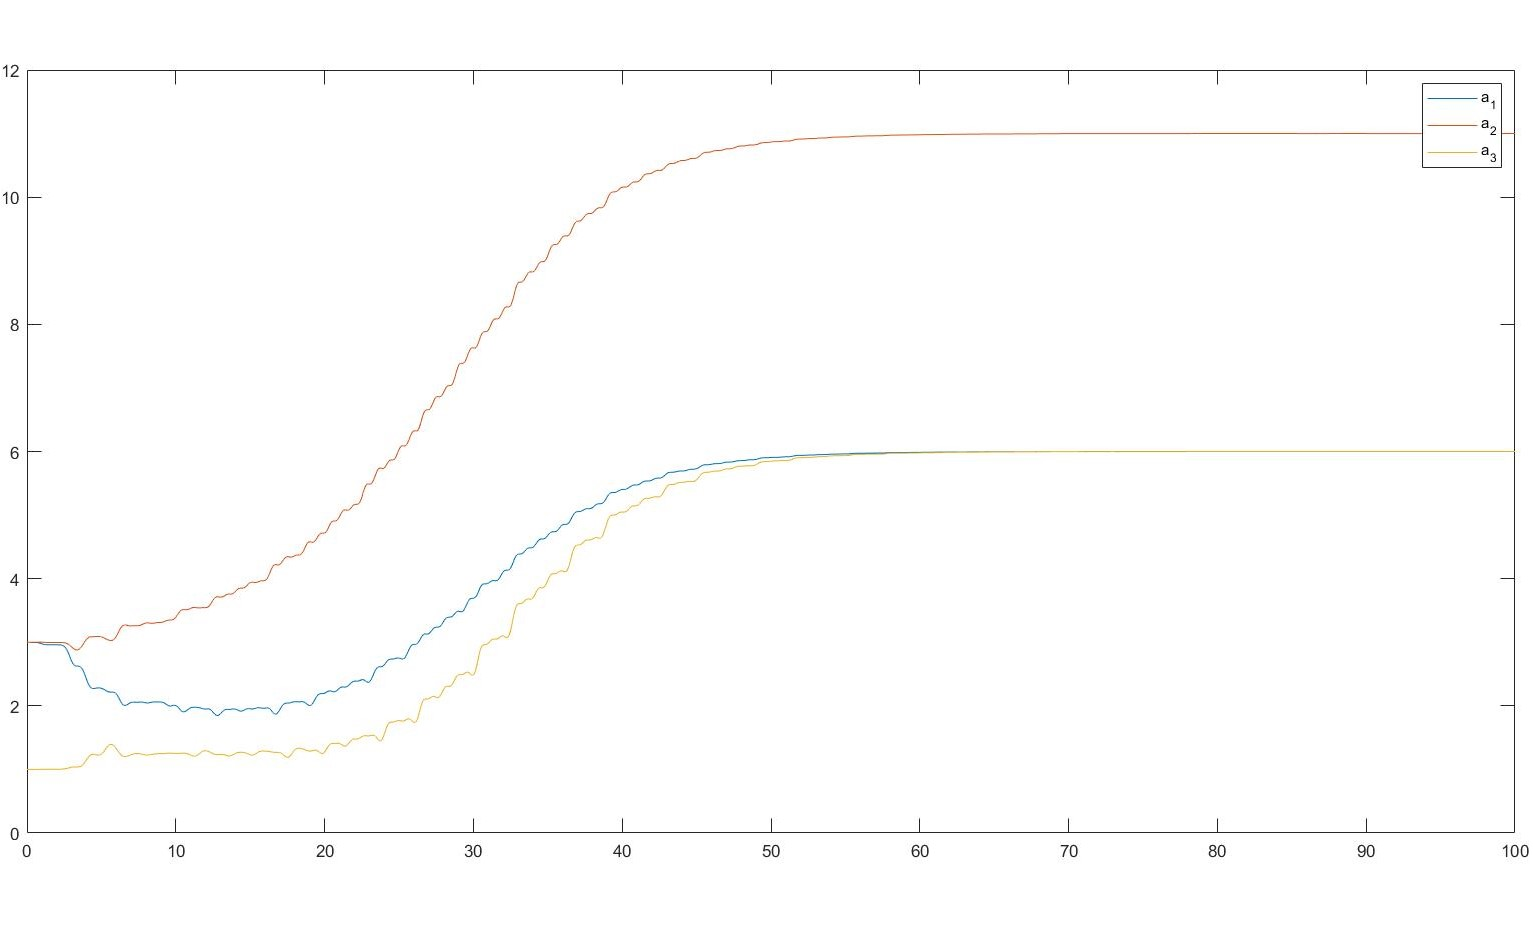
\includegraphics[width=\linewidth]{a_est_online.jpg}
\centerline{Σχήμα 3.5.1: Σύγκλιση Παραμέτρων $a$}
\\
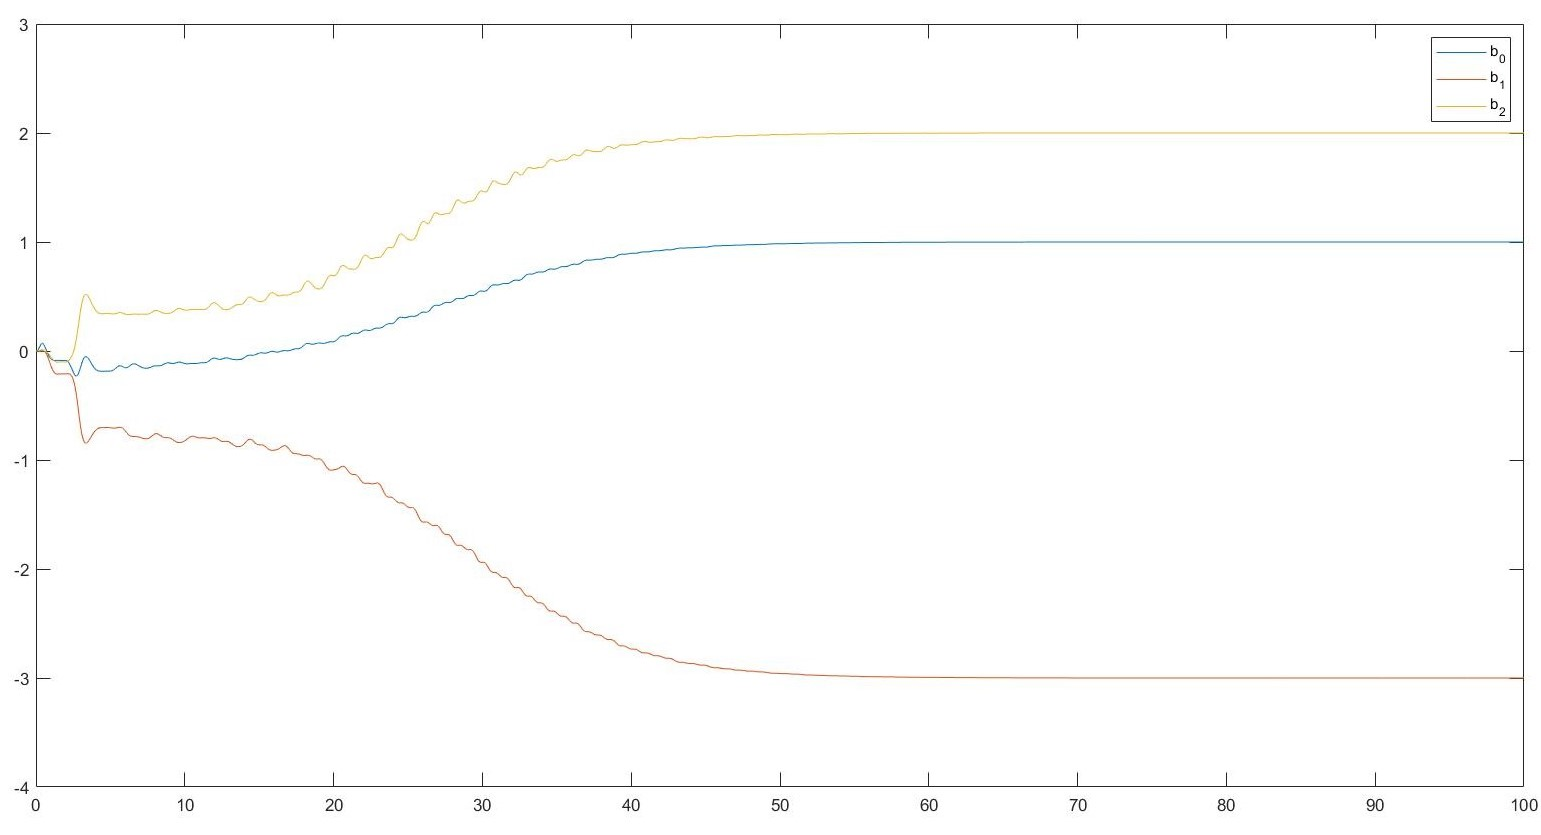
\includegraphics[width=\linewidth]{b_est_online.jpg}
\centerline{Σχήμα 3.5.2: Σύγκλιση Παραμέτρων $b$}
\\ \\
Και οι γραφικές παραστάσεις των σφαλμάτων $E$ φαίνονται για τις δύο μεθόδους αντίστοιχα παρακάτω
\\
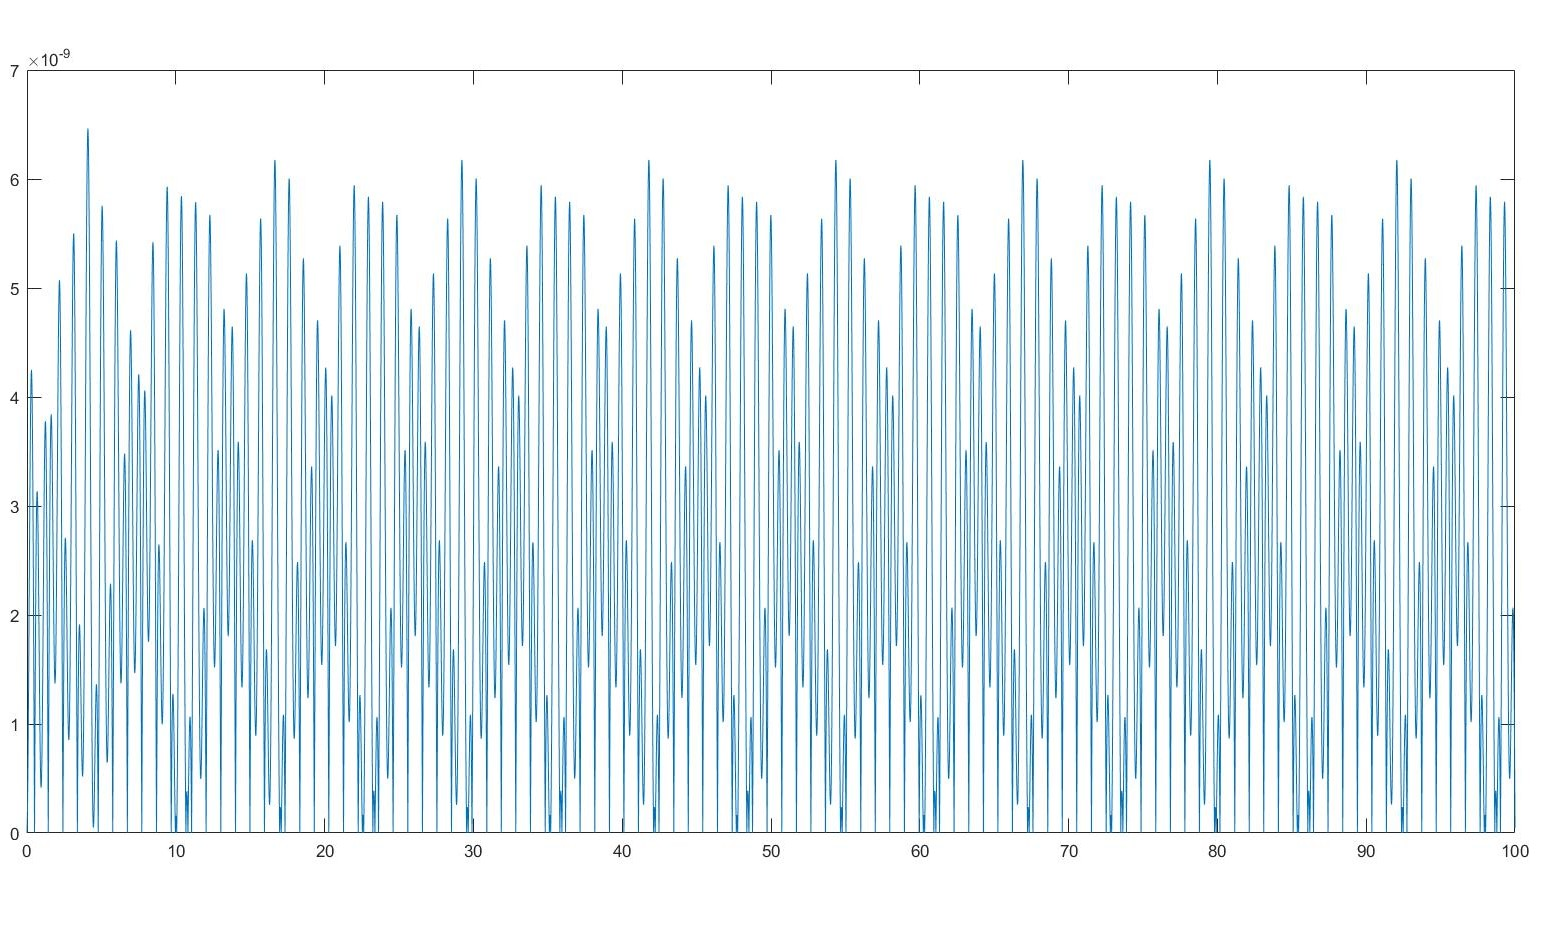
\includegraphics[width=\linewidth]{offline_error.jpg}
\centerline{Σχήμα 3.5.3: Σφάλμα Offline Μεθόδου Ελαχίστων Τετραγώνων}
\\
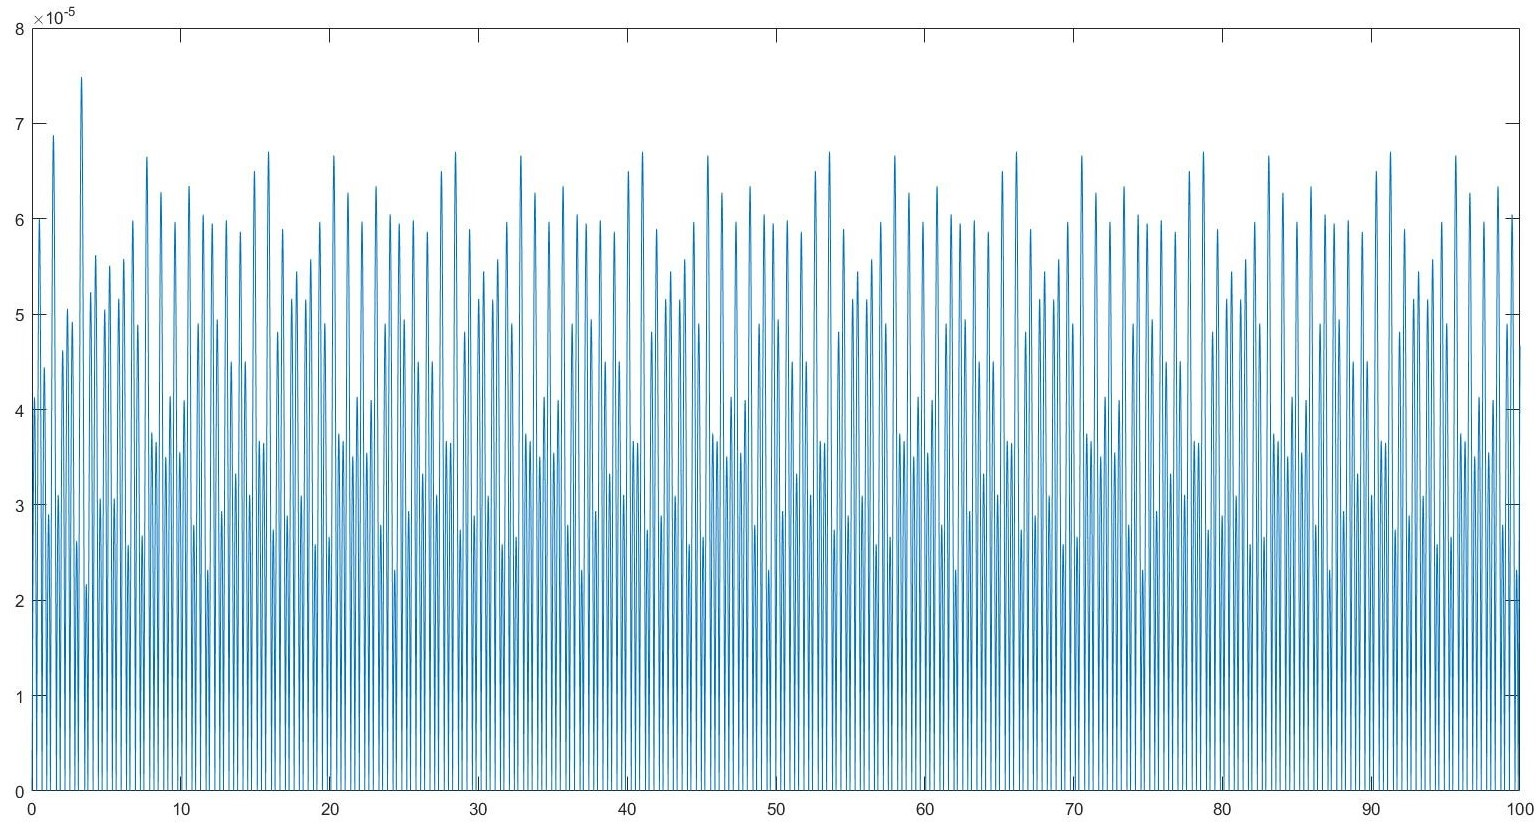
\includegraphics[width=\linewidth]{online_error.jpg}
\centerline{Σχήμα 3.5.4: Σφάλμα Online Μεθόδου Ελαχίστων Τετραγώνων}
\\ \\
Τέλος, αξίζει να παρατηρήσουμε ότι το σφάλμα-κριτήριο που χρησιμοποιήσαμε για την αξιολόγηση-επιλογή του τελικού μοντέλου είναι μικρότερο στην offline μέθοδο από ότι στην online.
\end{document}
